% !TeX program = pdflatex
% Artigo do TCC02 -- rascunho. O template oficial da coordenação para o TCC02 não está no
% repositório (ver Plano_Trabalho/LEIAM-ME.txt); as seções ficam em arquivos separados justamente
% pra poderem ser movidas para o template oficial sem retrabalho.
% Compilar: latexmk -pdf main.tex

\documentclass[a4paper,11pt]{article}

\usepackage[T1]{fontenc}
\usepackage[utf8]{inputenc}
\usepackage[english,brazil]{babel}
\usepackage{mathptmx}
\usepackage[top=25mm,bottom=25mm,left=25mm,right=25mm]{geometry}
\usepackage{setspace}\onehalfspacing
\usepackage{indentfirst}
\usepackage{graphicx}
\usepackage{booktabs}
\usepackage{array}
\usepackage{amsmath}
\usepackage{xcolor}
\usepackage{caption}
\captionsetup{font=small,labelfont=bf}
\setlength{\marginparwidth}{2cm}
\usepackage[disable]{todonotes} % trocar [disable] por [] pra ver as pendências marcadas no texto
\usepackage[hidelinks]{hyperref}

\graphicspath{{../Pesquisa/resultados/graficos/}}
\newcommand{\tabela}[1]{\input{../Pesquisa/resultados/tabelas/#1.tex}}

\title{Eficiência de métodos de RAG em documentos em português:\\
uma análise comparativa em domínios médico, financeiro e técnico-científico}
\author{
  Afonso Henriques Massunari \and Ryan Alves Mazzeu\\[2mm]
  \small Engenharia de Computação -- Universidade Federal de Itajubá (UNIFEI)\\[1mm]
  \small Orientador: Carlos Henrique Valério de Moraes
}
\date{}

\begin{document}

\maketitle

\begin{quote}
\small
\noindent\textbf{Resumo.} A Geração Aumentada por Recuperação (RAG) é a principal forma de ancorar respostas de modelos de linguagem em documentos, mas a escolha do método de injeção de contexto afeta custo e qualidade de maneiras pouco medidas fora do inglês. Este trabalho replica, com documentos em português, a comparação de seis métodos de RAG (Stuff, Refine, Map-Reduce, Map-Rerank, Query Step-Down e Reciprocal RAG) proposta por Şakar e Emekci (2025), em três domínios brasileiros com respostas de referência verificáveis: a prova discursiva do Revalida 2024/2, as Informações Trimestrais da Grendene S.A. e um artigo científico sobre RAG em português. As 162 respostas foram avaliadas por similaridade de cosseno e por quatro métricas RAGAS, com validação do juiz automático contra ele mesmo e contra um juiz de outra família de modelos. Também foram avaliados filtros de compressão contextual e o custo de infraestrutura de ChromaDB e FAISS. Nenhum método foi estatisticamente superior em similaridade de cosseno, enquanto o custo variou até cinco vezes entre eles. A ordenação dos métodos mudou com a métrica: o Map-Rerank teve a maior similaridade de cosseno e uma das menores \emph{Answer Relevancy}. O método mais simples, o Stuff, recusou 30\% das perguntas, na maioria das vezes com a informação presente no contexto recuperado. Limiares fixos de compressão ou não tiveram efeito, ou descartaram quase todo o contexto, enquanto limiares calibrados na distribuição de similaridade reduziram cerca de 40\% dos tokens sem perda de qualidade em dois dos três domínios. Os resultados indicam que a escolha do método em RAG é sobretudo uma decisão de custo e do tipo de resposta esperada, e que conclusões baseadas em uma única métrica automática devem ser vistas com cautela.

\medskip
\noindent\textbf{Palavras-chave:} geração aumentada por recuperação; modelos de linguagem; avaliação de RAG; RAGAS; compressão contextual; português.

\bigskip
\noindent\textbf{Abstract.} Retrieval-Augmented Generation (RAG) is the main way to ground language model answers in documents, but the choice of context injection method affects cost and quality in ways rarely measured outside English. This work replicates, with Portuguese documents, the comparison of six RAG methods (Stuff, Refine, Map-Reduce, Map-Rerank, Query Step-Down and Reciprocal RAG) proposed by Şakar and Emekci (2025), in three Brazilian domains with verifiable reference answers: the Revalida 2024/2 medical licensing exam, the quarterly financial statements of Grendene S.A., and a scientific paper on RAG in Portuguese. The 162 answers were evaluated with cosine similarity and four RAGAS metrics, and the automatic judge was validated against itself and against a judge from another model family. Contextual compression filters and the infrastructure cost of ChromaDB and FAISS were also evaluated. No method was statistically superior in cosine similarity, while cost varied up to fivefold across methods. The ranking of methods changed with the metric: Map-Rerank had the highest cosine similarity and one of the lowest Answer Relevancy scores. The simplest method, Stuff, refused to answer 30\% of the questions, mostly when the information was present in the retrieved context. Fixed compression thresholds either had no effect or discarded almost all context, whereas thresholds calibrated on the similarity distribution cut about 40\% of tokens without quality loss in two of the three domains. The results indicate that choosing a RAG method is mainly a decision about cost and the expected answer type, and that conclusions based on a single automatic metric should be taken with caution.

\medskip
\noindent\textbf{Keywords:} retrieval-augmented generation; language models; RAG evaluation; RAGAS; contextual compression; Portuguese.
\end{quote}

\section{Introdução}
\label{sc:introducao}

Os Modelos de Linguagem de Grande Porte (LLMs) ampliaram de forma expressiva o alcance de sistemas de processamento de linguagem natural, mas continuam sujeitos a alucinações e ao envelhecimento do conhecimento aprendido durante o treinamento. A Geração Aumentada por Recuperação (RAG) \cite{lewis2020rag} consolidou-se como a principal alternativa não-paramétrica para mitigar esse problema \cite{andriopoulos2023augmenting}: em vez de depender apenas do conhecimento interno do modelo, o sistema recupera trechos relevantes de uma base documental, indexada em um banco de dados vetorial \cite{ma2024vectorsurvey}, e os fornece ao LLM no momento da geração. Na prática, porém, um pipeline RAG envolve uma sequência de escolhas de engenharia --- o método de injeção do contexto, o banco vetorial, o modelo de embedding, filtros de compressão --- cujo efeito combinado sobre qualidade da resposta, consumo de tokens e tempo de execução raramente é medido de forma sistemática.

Şakar e Emekci \cite{sakar2025rag} realizaram a análise mais abrangente desse espaço de decisão: uma busca em grade com 23.625 configurações, cruzando seis métodos de RAG (Stuff, Refine, Map-Reduce, Map-Rerank, Query Step-Down e Reciprocal RAG), três bancos vetoriais, três modelos de embedding, três LLMs e filtros de compressão contextual, sobre três domínios em inglês --- relatórios financeiros (SEC 10-Q), documentação técnico-científica (artigo do Llama 2) e questões médicas (MedQA). O estudo mostra que não há arquitetura universalmente ótima: o Reciprocal RAG obteve a maior similaridade com as respostas de referência, enquanto o Stuff foi o mais rápido e o mais econômico em tokens.

Esses resultados, no entanto, foram obtidos exclusivamente com documentos em inglês e avaliados por uma única métrica de qualidade, a similaridade de cosseno entre resposta gerada e resposta de referência. Não se sabe se as mesmas conclusões se sustentam em português, idioma em que a literatura de avaliação de RAG ainda é escassa \cite{medeiros2025embeddings}, nem se a escolha da métrica altera a ordenação dos métodos. Este trabalho investiga essas duas questões. Mantém-se a estrutura comparativa do estudo de referência --- os mesmos seis métodos, o mesmo tamanho de fragmento e a mesma lógica de compressão por limiar de similaridade ---, mas os três domínios em inglês são substituídos por equivalentes brasileiros com respostas de referência oficiais ou ancoradas literalmente no texto-fonte: a prova discursiva do Revalida 2024/2 (INEP) no domínio médico, as Informações Trimestrais da Grendene S.A. (CVM/B3) no domínio financeiro e um artigo científico brasileiro sobre RAG em português \cite{medeiros2025embeddings} no domínio técnico-científico.

O trabalho busca responder às seguintes questões de pesquisa:

\begin{enumerate}
  \item[\textbf{QP1.}] Como os seis métodos de RAG se comparam em qualidade de resposta e em custo (tokens e tempo) sobre documentos em português?
  \item[\textbf{QP2.}] A ordenação dos métodos depende da métrica de qualidade adotada --- similaridade de cosseno ou métricas do \emph{framework} RAGAS \cite{es2024ragas}?
  \item[\textbf{QP3.}] Qual é o compromisso entre economia de tokens e perda de qualidade da compressão contextual por limiar de similaridade, e limiares fixos são transferíveis entre domínios?
  \item[\textbf{QP4.}] Como ChromaDB e FAISS se comparam em custo de infraestrutura quando operam sobre os mesmos vetores?
\end{enumerate}

Como questão metodológica transversal, verifica-se ainda se o juiz automático das métricas RAGAS --- o mesmo LLM que gera as respostas --- concorda com um juiz independente de outra família de modelos, dado o risco conhecido de viés de autopreferência em avaliações por LLM \cite{zheng2023judging, panickssery2024selfpref}.

O restante do artigo está organizado da seguinte forma. A Seção~\ref{sc:fundamentacao} apresenta a fundamentação teórica e os trabalhos relacionados. A Seção~\ref{sc:metodos} descreve os corpora, o pipeline, as métricas e a análise estatística. A Seção~\ref{sc:resultados} apresenta os resultados, discutidos na Seção~\ref{sc:discussao} junto com as limitações do estudo. A Seção~\ref{sc:conclusao} conclui o trabalho.

\section{Fundamentação e trabalhos relacionados}
\label{sc:fundamentacao}

\subsection{Geração aumentada por recuperação}

Na formulação de Lewis et al.~\cite{lewis2020rag}, um sistema RAG combina um componente de recuperação, que seleciona trechos de uma coleção de documentos a partir da pergunta, e um componente gerador, que condiciona a resposta a esses trechos. Em implementações atuais, os documentos são divididos em fragmentos (\emph{chunks}) \cite{schwaber2025chunking}, convertidos em vetores por um modelo de embedding e armazenados em um banco vetorial \cite{ma2024vectorsurvey}; a pergunta é codificada pelo mesmo modelo, e os $k$ fragmentos mais próximos são entregues ao LLM. A arquitetura reduz alucinações e permite atualizar o conhecimento sem retreinar o modelo \cite{andriopoulos2023augmenting}, mas sua robustez depende de decisões tomadas empiricamente: Barnett et al.~\cite{barnett2024seven} catalogam sete pontos de falha recorrentes, entre eles a recuperação de trechos errados e a incapacidade do gerador de extrair a resposta de um contexto que a contém.

\subsection{Métodos de injeção de contexto}

Uma vez recuperados os fragmentos, há diferentes formas de entregá-los ao LLM \cite{topsakal2023langchain}. No \textbf{Stuff}, todos os fragmentos são concatenados em um único prompt. No \textbf{Refine}, a resposta é construída a partir do primeiro fragmento e refinada sequencialmente a cada fragmento seguinte. No \textbf{Map-Reduce}, cada fragmento gera uma resposta parcial independente, e uma chamada final combina as parciais. No \textbf{Map-Rerank}, cada fragmento gera uma resposta acompanhada de uma nota de confiança, e mantém-se apenas a de maior confiança. Şakar e Emekci~\cite{sakar2025rag} acrescentam dois métodos que atuam sobre a pergunta: o \textbf{Query Step-Down} gera perguntas alternativas mais específicas, responde cada uma e combina as respostas; o \textbf{Reciprocal RAG} segue o mesmo primeiro passo, mas retém apenas a resposta mais confiável. Ambos dialogam com a reescrita de consultas \cite{ma2023query} e com o RAG-Fusion \cite{rackauckas2024ragfusion}, que ampliam a cobertura da recuperação ao custo de chamadas adicionais ao LLM e do risco de desvio em relação à intenção original da pergunta.

A escolha do método tem efeito direto sobre o número de chamadas ao LLM e, portanto, sobre tokens e latência. Há também um efeito sobre a qualidade: Liu et al.~\cite{liu2023lost} mostram que LLMs aproveitam pior a informação posicionada no meio de contextos longos, o que penaliza estratégias que apenas acumulam fragmentos, e Nair et al.~\cite{nair2023drilling} mostram que representações condensadas de documentos longos preservam quase todo o desempenho com uma fração dos tokens.

\subsection{Compressão contextual e bancos vetoriais}

A compressão contextual reduz o volume de texto enviado ao LLM descartando fragmentos pouco relevantes. Em sua forma mais simples, adotada por Şakar e Emekci~\cite{sakar2025rag}, descartam-se os fragmentos cuja similaridade com a pergunta fica abaixo de um limiar. Os autores observaram economia de recursos, mas também queda de qualidade quando o limiar é punitivo demais para o domínio. Quanto à camada de armazenamento, bancos como o ChromaDB oferecem persistência em disco e filtros por metadados, enquanto bibliotecas como o FAISS \cite{johnson2021faiss} priorizam a velocidade da busca por similaridade em memória. Como ambos podem operar sobre os mesmos vetores com a mesma métrica de distância, a diferença entre eles é essencialmente de infraestrutura, e não de qualidade de recuperação.

\subsection{Avaliação de sistemas RAG}

A similaridade de cosseno entre os embeddings da resposta gerada e da resposta de referência é uma métrica barata e reprodutível, mas mede proximidade semântica global: penaliza respostas corretas redigidas de forma mais longa que a referência e não verifica se a resposta está ancorada nos documentos recuperados. O \emph{framework} RAGAS \cite{es2024ragas} propõe métricas específicas para RAG calculadas com um LLM como juiz: \emph{Faithfulness} (fração das afirmações da resposta sustentadas pelo contexto recuperado), \emph{Answer Relevancy} (quanto a resposta endereça a pergunta), \emph{Context Precision} e \emph{Context Recall} (qualidade e suficiência do contexto recuperado em relação à referência). O uso de LLMs como juízes, porém, tem vieses documentados, entre eles o de autopreferência: juízes tendem a avaliar melhor textos gerados por eles mesmos \cite{zheng2023judging, panickssery2024selfpref}. Isso é relevante quando, por restrição de orçamento, o mesmo modelo gera e avalia as respostas.

\subsection{RAG em português}

A avaliação de RAG em português ainda é incipiente. Medeiros e Oliveira~\cite{medeiros2025embeddings} compararam modelos de embedding e LLMs abertos e proprietários em três bases em português (Pirá, SQuAD 2 e FairytaleQA PT-BR), com ROUGE-L, BERTScore e as métricas RAGAS de fidelidade e relevância da resposta --- estas calculadas com o GPT-4o-mini como juiz e, por restrição orçamentária, apenas em duas das bases. Os melhores resultados foram obtidos pelo Multilingual E5 large e pelo Gemma 2 9B. Aquele estudo varia o embedding e o LLM com um método de injeção fixo; o presente trabalho faz o recorte complementar, fixando embedding e LLM e variando o método de injeção, a compressão contextual e o banco vetorial, sobre documentos longos de domínios profissionais.

\subsection{Lacuna}

A literatura avançou na acurácia \cite{ma2023query, rackauckas2024ragfusion}, na confiabilidade \cite{andriopoulos2023augmenting, barnett2024seven} e no entendimento das limitações de contexto \cite{liu2023lost, nair2023drilling} de sistemas RAG, e aplicações em domínios verticais --- jurídico \cite{cui2023chatlaw} e financeiro \cite{gupta2023gptinvestar} --- mostram a relevância prática do tema. A comparação sistemática entre métodos de injeção de contexto, porém, foi feita apenas em inglês \cite{sakar2025rag} e com uma única métrica de qualidade. Não há, até onde foi possível verificar, uma replicação desse desenho com documentos em português nem uma verificação de quanto as conclusões dependem da métrica escolhida. Este trabalho se insere nessa lacuna.

\section{Materiais e métodos}
\label{sc:metodos}

O estudo é quantitativo e experimental. O desenho segue o de Şakar e Emekci~\cite{sakar2025rag}, com os mesmos seis métodos de RAG e o mesmo tamanho de fragmento, mas com documentos e perguntas em português. Para isolar o efeito do método de injeção de contexto, o modelo de embedding, o LLM, o tamanho dos fragmentos e o número de fragmentos recuperados foram mantidos fixos em todos os experimentos.

\subsection{Corpora e perguntas}

Cada domínio do estudo de referência foi substituído por um equivalente brasileiro do mesmo tipo (Tabela~\ref{tab:corpora}). O critério comum aos três foi que toda resposta de referência tivesse fonte verificável: um gabarito oficial ou um trecho literal do documento. Nenhuma resposta de referência foi escrita a partir de conhecimento próprio dos autores.

\begin{table}[htbp]
\centering
\small
\caption{Domínios, documentos e perguntas utilizados.}
\label{tab:corpora}
\begin{tabular}{p{2.4cm}p{6.2cm}cc}
\toprule
Domínio & Documentos (corpus de recuperação) & Fragmentos & Perguntas \\
\midrule
Médico (Revalida) & Código de Ética Médica (CFM); guia \emph{Consulta do adolescente} (SBP); Diretriz de Tromboembolismo Venoso 2022; artigo Febrasgo sobre as recomendações da OMS (2018) para o parto; Guia de Vigilância em Saúde, cap. Doença Meningocócica (MS) & 430 & 12 \\
Financeiro (Grendene) & Informações Trimestrais (ITR) de 30/09/2025 da Grendene S.A. \cite{grendene2025itr} & 199 & 7 \\
Técnico-científico (SBC) & Artigo de Medeiros e Oliveira~\cite{medeiros2025embeddings} & 42 & 8 \\
\midrule
Total & & 671 & 27 \\
\bottomrule
\end{tabular}
\end{table}

\textbf{Médico.} As perguntas são os subitens das Questões 1, 3, 4 e 5 da prova discursiva do Revalida 2024/2, e as respostas de referência são o padrão de resposta definitivo publicado pelo INEP \cite{inep2024revalida}. O corpus de recuperação é formado pelos documentos citados na referência bibliográfica do próprio gabarito, reunidos em um único índice: para cada pergunta, o recuperador precisa encontrar o documento certo entre os cinco. A Questão 2 foi excluída porque sua única referência é o manual do curso ATLS, material pago e protegido por direitos autorais, e um subitem que dependia da interpretação de uma imagem também foi excluído. A pergunta enviada ao sistema é a vinheta clínica seguida do enunciado do subitem.

\textbf{Financeiro.} O documento é o relatório trimestral oficial da Grendene S.A., com balanço patrimonial, demonstrações de resultado e de fluxo de caixa e notas explicativas (72 páginas). Como o documento não traz perguntas, as sete perguntas foram redigidas pelos autores, cada uma ancorada em um trecho literal do relatório (por exemplo, a taxa de câmbio de fechamento do dólar e o lucro líquido consolidado do trimestre).

\textbf{Técnico-científico.} O documento é o artigo de Medeiros e Oliveira~\cite{medeiros2025embeddings}, escolhido por ser um texto científico brasileiro sobre o próprio tema deste trabalho. As oito perguntas seguem o mesmo procedimento do domínio financeiro.

Os PDFs foram convertidos em texto simples antes da fragmentação. Os arquivos originais, os textos extraídos e as perguntas com suas respostas de referência estão disponíveis no repositório do trabalho.

\subsection{Pipeline}

Os documentos foram divididos com o \texttt{RecursiveCharacterTextSplitter} (fragmentos de 1.000 caracteres com sobreposição de 100, os mesmos valores do estudo de referência) e codificados com o BGE-M3 \cite{chen2024bgem3}, modelo de embedding multilíngue, usando apenas os vetores densos. O BGE-small em inglês, usado pelo estudo de referência, foi substituído por não suportar português. Os vetores foram indexados no ChromaDB com distância euclidiana. Como os vetores são normalizados, a similaridade de cosseno entre pergunta e fragmento é obtida diretamente da distância quadrática $d^2$ retornada pelo banco, como $\cos = 1 - d^2/2$. Em todos os métodos, a recuperação devolve os $k = 4$ fragmentos mais próximos.

A geração foi feita com o \texttt{gpt-4o-mini} da OpenAI, com temperatura 0, um dos três LLMs avaliados por Şakar e Emekci~\cite{sakar2025rag}. O identificador \texttt{gpt-4o-mini} é um apelido que a API resolve para uma versão específica do modelo. Na data de redação deste artigo, ele correspondia a \texttt{gpt-4o-mini-2024-07-18}; os registros dos experimentos armazenaram apenas o apelido.\todo{Confirmar se dá pra afirmar a versão usada nos experimentos (setembro/2026).}

Os seis métodos foram implementados diretamente sobre a API, sem uso de \emph{frameworks} de orquestração, para que cada chamada ao LLM fosse contabilizada:

\begin{itemize}
  \item \textbf{Stuff} (1 chamada): os $k$ fragmentos são concatenados em um único prompt, com a instrução ``Responda à pergunta usando apenas o contexto abaixo. Se a resposta não estiver no contexto, diga que não sabe.''
  \item \textbf{Refine} ($k$ chamadas): gera uma resposta com o primeiro fragmento e a refina com cada fragmento seguinte, alterando-a apenas se o novo fragmento trouxer informação relevante.
  \item \textbf{Map-Reduce} ($k+1$ chamadas): gera uma resposta parcial por fragmento e combina as parciais em uma resposta final.
  \item \textbf{Map-Rerank} ($k$ chamadas): gera, para cada fragmento isoladamente, uma resposta e uma nota de confiança de 0 a 100, e mantém a resposta de maior confiança.
  \item \textbf{Query Step-Down} (6 chamadas): a partir da pergunta e de um contexto inicial, gera quatro perguntas alternativas mais específicas, responde cada uma com Stuff e combina as quatro respostas. O estudo de referência não deixa explícito se a combinação usa uma chamada própria ao LLM; aqui optou-se por usá-la.
  \item \textbf{Reciprocal RAG} (5 chamadas): gera as mesmas quatro perguntas alternativas, responde cada uma com nota de confiança e mantém a resposta mais confiável, sem etapa de combinação.
\end{itemize}

\subsection{Métricas}

\textbf{Similaridade de cosseno.} É a métrica de qualidade do estudo de referência: a similaridade de cosseno entre os embeddings BGE-M3 da resposta gerada e da resposta de referência.

\textbf{RAGAS.} Foram calculadas quatro métricas do RAGAS \cite{es2024ragas} (biblioteca \texttt{ragas} 0.4.3): \emph{Answer Relevancy}, \emph{Faithfulness}, \emph{Context Precision} e \emph{Context Recall}. O juiz foi o próprio \texttt{gpt-4o-mini}, com limite de 4.096 tokens de saída, e o embedding da \emph{Answer Relevancy} foi o \texttt{text-embedding-3-small} da OpenAI. As três últimas métricas avaliam o conjunto de fragmentos entregue ao gerador e só se aplicam aos quatro métodos que recebem esse conjunto. O Query Step-Down e o Reciprocal RAG fazem uma recuperação por pergunta alternativa, sem um conjunto único a avaliar, e por isso recebem apenas a \emph{Answer Relevancy}. Avaliações que falharam (por exemplo, por saída truncada do juiz) foram registradas como ausentes, e não imputadas.

\textbf{Validação do juiz.} Como o mesmo modelo gera e avalia as respostas, há risco de viés de autopreferência \cite{panickssery2024selfpref}. Para estimá-lo, uma amostra estratificada de 54 respostas (3 por combinação de domínio e método, sorteadas com semente fixa) foi avaliada novamente por dois juízes: um juiz independente de outra família de modelos, o Command A da Cohere (\texttt{command-a-03-2025}), sucessor do Command-R avaliado pelo estudo de referência, com as mesmas métricas e o mesmo embedding; e o próprio \texttt{gpt-4o-mini}, uma segunda vez, para medir a variação do juiz consigo mesmo. A comparação entre as duas medidas indica se a discordância com o juiz independente é maior do que o ruído de uma única avaliação.

\textbf{Custo.} Para cada pergunta, foram registrados os tokens de entrada e de saída informados pela API e o tempo total, da recuperação até o fim da geração. O uso de CPU e memória também foi registrado com a biblioteca \texttt{psutil}, mas não é analisado aqui: como a geração ocorre nos servidores da API, essas medidas refletem apenas o cliente, e não o custo de inferência do método.

\subsection{Compressão contextual}

O filtro de compressão descarta, antes da geração, os fragmentos recuperados cuja similaridade com a pergunta fica abaixo de um limiar. Se todos ficarem abaixo, o fragmento mais similar é mantido. O filtro foi aplicado ao método Stuff, o de menor custo, com as mesmas 27 perguntas, em duas rodadas: com limiares fixos de 0,3, 0,5 e 0,7; e com limiares calibrados por domínio, definidos como os quantis 25, 50 e 75 da similaridade dos fragmentos do top-4 de todas as perguntas do domínio. A segunda rodada foi motivada pelo resultado da primeira (Seção~\ref{sc:resultados}). Como a calibração usa as mesmas perguntas avaliadas, os limiares calibrados medem o efeito de descartar uma fração controlada dos fragmentos, e não o desempenho de um limiar escolhido de antemão.

\subsection{Bancos vetoriais}

O ChromaDB (persistente em disco) foi comparado ao FAISS \cite{johnson2021faiss} (\texttt{IndexFlatL2}, busca exata em memória) sobre os mesmos vetores BGE-M3 dos três domínios, medindo tempo de indexação, tempo médio de consulta, memória alocada na indexação e concordância entre os fragmentos do top-$k$ retornados pelos dois bancos. Como a busca é exata nos dois casos e a métrica de distância é a mesma, a qualidade das respostas não depende do banco, e a comparação se restringe à infraestrutura. As medições foram feitas em processos separados para os dois bancos, sem chamadas ao LLM.

\subsection{Análise estatística}

As 27 perguntas foram tratadas como blocos pareados, já que todos os métodos respondem às mesmas perguntas. A diferença entre métodos foi testada com o teste de Friedman e, em seguida, com testes de Wilcoxon pareados par a par, com os valores-$p$ corrigidos pelo método de Holm \cite{holm1979simple}, seguindo a recomendação de Demšar~\cite{demsar2006statistical} para comparação de vários métodos sobre as mesmas instâncias. Intervalos de confiança de 95\% das médias foram estimados por \emph{bootstrap} percentil (10.000 reamostragens), e as correlações entre métricas e entre juízes, pelo coeficiente de Spearman. O nível de significância adotado foi 0,05. Com 27 perguntas, os testes têm baixo poder: a ausência de significância indica que a diferença não pode ser afirmada com esta amostra, e não que ela seja nula.

\subsection{Ambiente e reprodutibilidade}

Os experimentos foram executados em Python 3.12 em um notebook com processador Intel Core i5-12450H (12 \emph{threads}), cerca de 20 GB de RAM e sem GPU dedicada; os embeddings foram calculados na CPU.\todo{Confirmar que todos os experimentos rodaram nesta máquina.} As principais bibliotecas foram \texttt{chromadb} 1.5.9, \texttt{faiss} 1.14.3, \texttt{FlagEmbedding} 1.4.0, \texttt{openai} 2.41.1, \texttt{ragas} 0.4.3 e \texttt{scipy} 1.17.1. Cada execução foi registrada em um arquivo JSONL, com pergunta, fragmentos recuperados, resposta, tokens, tempos e métricas. O código, os registros e o script que gera todas as tabelas e figuras deste artigo estão no repositório do trabalho.

\subsection{Diferenças em relação ao plano de trabalho}

O plano de trabalho aprovado no TCC01 previa os três conjuntos de dados em inglês do estudo de referência, os bancos ChromaDB, FAISS e Pinecone, três modelos de embedding (BGE-small, text-embedding-3-large e Cohere-en-v3) e métricas de similaridade de cosseno e RAGAS. Durante a execução, verificou-se que o desenho original reproduziria quase integralmente o estudo de referência, já publicado. Por isso, com a concordância do orientador, os conjuntos de dados foram substituídos por equivalentes em português, o que define a contribuição do trabalho. O embedding foi fixado no BGE-M3, único dos modelos considerados com suporte adequado a português e execução local sem custo, e o Pinecone, serviço pago em nuvem, não foi incluído. Essas escolhas reduzem o espaço de configurações em relação ao estudo de referência, mas mantêm o eixo central de comparação: os seis métodos de RAG, a compressão contextual e o custo de infraestrutura dos bancos vetoriais.\todo{Revisar com o orientador a redação da justificativa.}

\section{Resultados}
\label{sc:resultados}

\subsection{Qualidade e custo dos seis métodos}
\label{ssc:metodos}

A Tabela~\ref{tab:similaridade_metodos} apresenta a similaridade de cosseno média por domínio e método nas 162 execuções (27 perguntas $\times$ 6 métodos), e a Figura~\ref{fig:similaridade_metodos} mostra as médias gerais com seus intervalos de confiança. O Map-Rerank obteve a maior média geral (0,744), seguido de um grupo praticamente empatado formado por Map-Reduce e Query Step-Down (0,682), Reciprocal (0,676), Refine (0,657) e Stuff (0,647). Os intervalos de confiança, porém, se sobrepõem amplamente, e o teste de Friedman não rejeita a hipótese de igualdade entre os métodos ($\chi^2 = 7{,}21$; $p = 0{,}205$). Nas comparações par a par, as menores diferenças brutas foram Map-Rerank contra Refine ($p = 0{,}017$) e contra Stuff ($p = 0{,}026$), mas nenhuma se mantém após a correção de Holm ($p_{\text{Holm}} \geq 0{,}26$; Tabela~\ref{tab:posthoc_similaridade}).

\tabela{similaridade_metodos}

\tabela{posthoc_similaridade}

\begin{figure}[htbp]
\centering
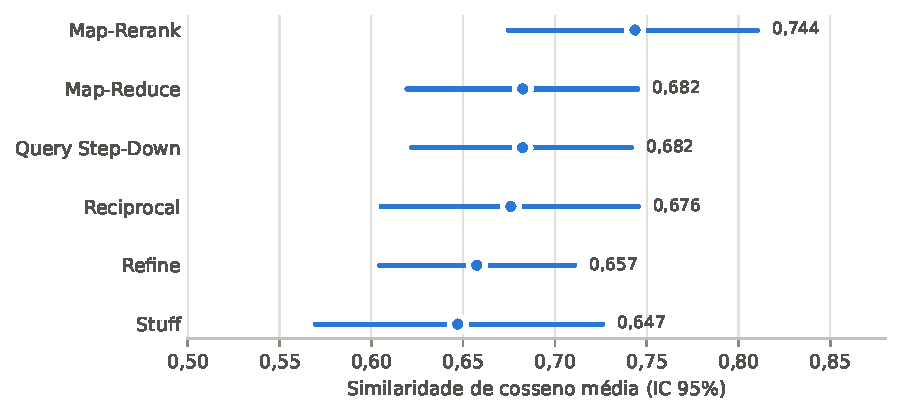
\includegraphics[width=0.78\linewidth]{similaridade_metodos.pdf}
\caption{Similaridade de cosseno média por método nas 27 perguntas, com intervalo de confiança de 95\% (\emph{bootstrap}).}
\label{fig:similaridade_metodos}
\end{figure}

A ordenação muda de um domínio para outro (Figura~\ref{fig:similaridade_heatmap}). O Map-Rerank lidera no domínio médico (0,714), o Reciprocal no financeiro (0,780) e o Stuff no técnico-científico (0,825) --- justamente o método com a pior média no domínio médico (0,555). Não há, portanto, um método que seja o melhor nos três domínios.

\begin{figure}[htbp]
\centering
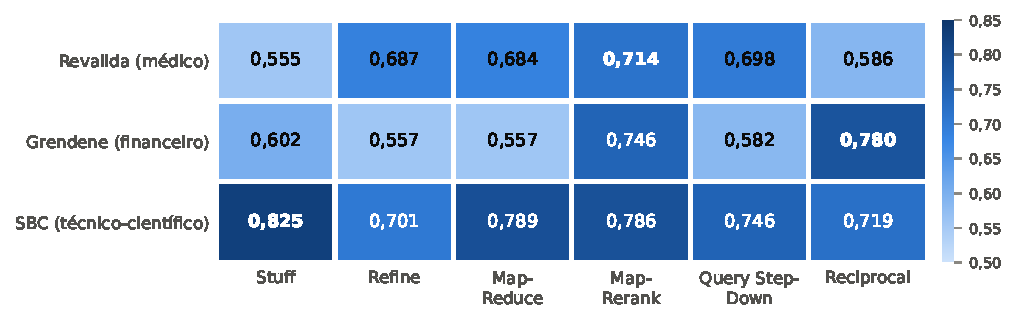
\includegraphics[width=0.95\linewidth]{similaridade_heatmap.pdf}
\caption{Similaridade de cosseno média por domínio e método. Em negrito, o melhor método de cada domínio.}
\label{fig:similaridade_heatmap}
\end{figure}

Em custo, as diferenças são grandes e sistemáticas (Tabela~\ref{tab:custo_metodos} e Figura~\ref{fig:custo_qualidade}). O Stuff é o mais barato (1.313 tokens e 3,4 s por pergunta, em média). Map-Rerank e Map-Reduce custam cerca de 1,5 vez o Stuff em tokens, e o Refine, 1,9 vez. Query Step-Down e Reciprocal, que geram e respondem quatro perguntas alternativas, custam cerca de 5 vezes o Stuff em tokens sem superar em qualidade os métodos mais baratos. O Map-Rerank combina a maior similaridade média com um custo próximo ao dos métodos intermediários.

\tabela{custo_metodos}

\begin{figure}[htbp]
\centering
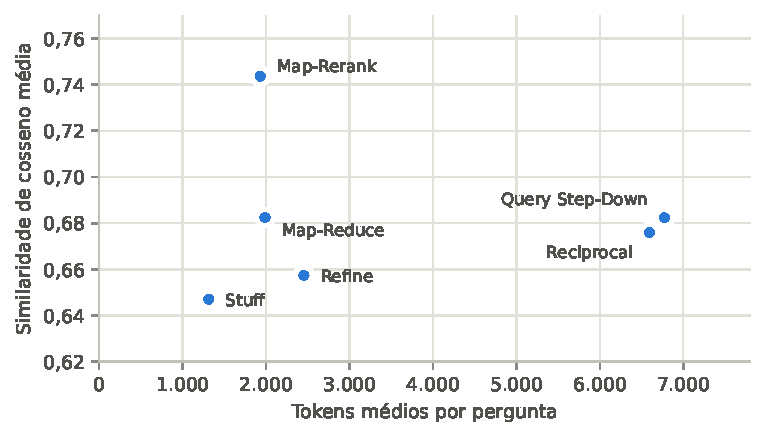
\includegraphics[width=0.72\linewidth]{custo_qualidade.pdf}
\caption{Custo médio em tokens por pergunta e similaridade de cosseno média de cada método.}
\label{fig:custo_qualidade}
\end{figure}

\subsection{Recusas}
\label{ssc:recusas}

Parte da diferença de qualidade vem das respostas em que o modelo declarou não ter a informação (Tabela~\ref{tab:recusas}). O prompt do Stuff instrui o modelo a dizer que não sabe quando a resposta não estiver no contexto, e o Stuff recusou 8 das 27 perguntas (30\%), seis delas no domínio médico. As 17 recusas observadas no total têm similaridade média de 0,436, contra 0,710 das demais respostas. Excluídas as recusas, a similaridade média do Stuff sobe de 0,647 para 0,746, praticamente a mesma do Map-Rerank sem recusas (0,758). O Map-Rerank recusou apenas uma vez: como cada fragmento gera uma resposta própria, com nota de confiança, basta que um dos quatro fragmentos sustente uma resposta para que ela prevaleça sobre as recusas dos demais. Nas oito perguntas recusadas pelo Stuff, o Map-Rerank respondeu sete, com similaridade maior em todas as sete.\todo{Conferir se a hipótese do mecanismo está bem formulada.}

\tabela{recusas}

A similaridade de cosseno também reage à forma da resposta, e não só ao seu conteúdo. Na pergunta sobre a taxa de câmbio do dólar (Grendene), Stuff, Refine e Map-Reduce responderam o valor correto (5,3186) em uma frase completa e obtiveram similaridade de 0,439, enquanto Map-Rerank e Reciprocal responderam apenas o número e obtiveram 1,0. Na direção oposta, na pergunta sobre o patrimônio líquido consolidado, o Map-Rerank respondeu 4.040.946 mil reais, valor diferente do gabarito (4.050.731), e ainda assim obteve similaridade de 0,613. Métodos que produzem respostas curtas, como Map-Rerank e Reciprocal, tendem a ser favorecidos pela métrica em perguntas factuais, estejam as respostas certas ou não.

\subsection{Métricas RAGAS}
\label{ssc:ragas}

A Tabela~\ref{tab:ragas_metodos} e a Figura~\ref{fig:ragas_heatmap} apresentam as métricas RAGAS das 162 respostas, todas avaliadas sem falhas. A \emph{Answer Relevancy} é a única métrica em que os métodos diferem de forma significativa (Friedman: $\chi^2 = 55{,}85$; $p < 0{,}001$), e sua ordenação é quase o inverso da obtida com a similaridade de cosseno. Query Step-Down (0,782), Map-Reduce (0,745) e Refine (0,706) lideram, e Map-Rerank (0,427) e Reciprocal (0,285) ficam nas últimas posições. Ou seja, os dois métodos favorecidos pelo cosseno são os mais penalizados. Nas comparações par a par, Query Step-Down, Map-Reduce e Refine superam Map-Rerank e Reciprocal com $p_{\text{Holm}} \leq 0{,}003$, e o Map-Reduce supera o Stuff ($p_{\text{Holm}} = 0{,}032$).

\tabela{ragas_metodos}

\begin{figure}[htbp]
\centering
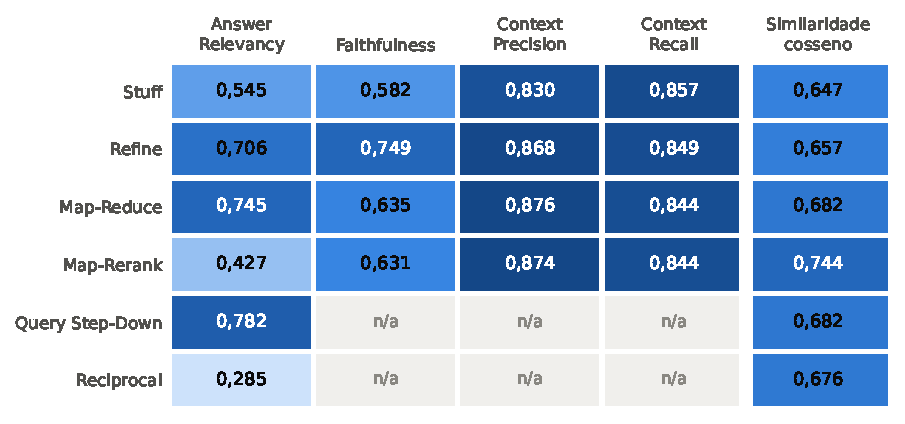
\includegraphics[width=0.85\linewidth]{ragas_heatmap.pdf}
\caption{Métricas RAGAS médias por método (juiz gpt-4o-mini) e similaridade de cosseno. As células cinzas indicam métricas que não se aplicam aos métodos com recuperação por pergunta alternativa.}
\label{fig:ragas_heatmap}
\end{figure}

A inversão decorre da forma como cada métrica trata respostas curtas. A \emph{Answer Relevancy} gera perguntas a partir da resposta e mede quanto elas se aproximam da pergunta original, atribuindo zero a respostas evasivas \cite{es2024ragas}. Uma resposta como ``5,3186'' ou ``Embolia pulmonar.'' gera perguntas pouco específicas e recebe nota baixa, enquanto a mesma resposta pode ter similaridade de cosseno alta com uma referência igualmente curta. Métodos que selecionam uma única resposta curta por nota de confiança, como Map-Rerank e Reciprocal, ficam no extremo oposto das duas métricas.

A \emph{Faithfulness} não difere significativamente entre os quatro métodos a que se aplica ($\chi^2 = 2{,}65$; $p = 0{,}449$). O Refine tem a maior média (0,749), mas a comparação é afetada pelas recusas: uma resposta como ``Não sei.'' não contém afirmações a verificar, e o juiz atribuiu \emph{Faithfulness} zero a 12 das 13 recusas. Excluídas as recusas, Stuff (0,827) e Refine (0,808) ficam à frente de Map-Reduce (0,666) e Map-Rerank (0,656). \emph{Context Precision} e \emph{Context Recall} variam pouco entre os métodos (0,83 a 0,88 e 0,84 a 0,86), o que era esperado: os quatro métodos recebem exatamente os mesmos fragmentos para cada pergunta, e a diferença entre eles está no uso do contexto, não na recuperação. Por isso mesmo, essas duas métricas deveriam ter valores idênticos entre os métodos, e as pequenas diferenças observadas medem a variação do próprio juiz (Seção~\ref{ssc:juiz}).

As métricas RAGAS confirmam a leitura das recusas da Seção~\ref{ssc:recusas}. Nas 13 recusas dos métodos com contexto, o \emph{Context Recall} médio foi de 0,744, e em 10 delas o juiz considerou que o contexto recuperado cobria ao menos metade da resposta de referência. Na maior parte das recusas, portanto, a informação estava disponível e o modelo não a usou.

A correlação entre a similaridade de cosseno e as métricas RAGAS, linha a linha, é fraca: $\rho = 0{,}20$ com a \emph{Answer Relevancy}, $0{,}35$ com a \emph{Faithfulness}, $0{,}16$ com a \emph{Context Precision} e $0{,}33$ com o \emph{Context Recall}. As métricas medem, em boa parte, coisas diferentes.

\subsection{Validação do juiz}
\label{ssc:juiz}

A Tabela~\ref{tab:concordancia_juizes} e a Figura~\ref{fig:concordancia_juizes} comparam, na amostra estratificada de 54 respostas, a avaliação principal do \texttt{gpt-4o-mini} com uma segunda avaliação do mesmo modelo (reteste) e com a avaliação do Command A. A confiabilidade variou bastante entre as métricas. Na \emph{Answer Relevancy}, o reteste reproduziu quase exatamente a avaliação principal ($\rho = 0{,}99$), e o juiz independente concordou em alto grau ($\rho = 0{,}93$), com a mesma ordenação dos seis métodos (Kendall $\tau = 1{,}00$). O \emph{Context Recall} também foi estável ($\rho = 0{,}84$ no reteste e $0{,}87$ entre juízes). Na \emph{Faithfulness}, a concordância foi moderada mesmo no reteste ($\rho = 0{,}76$) e menor entre juízes ($\rho = 0{,}57$). Na \emph{Context Precision}, os dois juízes praticamente não concordaram ($\rho = 0{,}03$), e o \texttt{gpt-4o-mini} deu notas mais altas (diferença média de $+0{,}18$; $p = 0{,}004$).

\tabela{concordancia_juizes}

\begin{figure}[htbp]
\centering
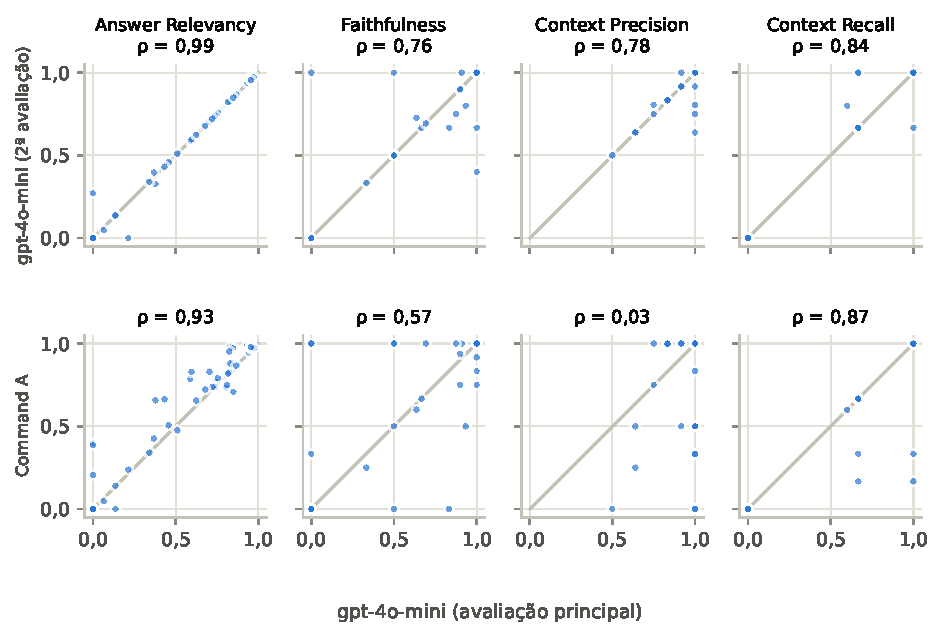
\includegraphics[width=0.95\linewidth]{concordancia_juizes.pdf}
\caption{Notas das métricas RAGAS na amostra de 54 respostas. Em cima, a avaliação principal do gpt-4o-mini (eixo horizontal) contra uma segunda avaliação do mesmo modelo; embaixo, contra o Cohere Command A. A diagonal indica concordância perfeita.}
\label{fig:concordancia_juizes}
\end{figure}

Nas métricas que avaliam a resposta gerada, não houve indício de autopreferência: o \texttt{gpt-4o-mini} deu às próprias respostas notas iguais ou menores que as do juiz independente, tanto na \emph{Answer Relevancy} (diferença média de $-0{,}050$; $p < 0{,}001$) quanto na \emph{Faithfulness} ($-0{,}038$; $p = 0{,}616$). As recusas foram tratadas de forma diferente pelos dois juízes: nas 7 recusas da amostra, a \emph{Faithfulness} média foi de 0,08 pelo \texttt{gpt-4o-mini} e de 0,33 pelo Command A.

O próprio comparativo oferece uma segunda medida da variação do juiz. Como os quatro métodos com contexto recebem os mesmos fragmentos, a \emph{Context Precision} e o \emph{Context Recall} de uma pergunta deveriam ser idênticos nos quatro. Isso ocorreu em 21 das 27 perguntas para a \emph{Context Precision} e em 24 para o \emph{Context Recall}. Nas demais, a nota variou entre avaliações da mesma entrada, em um caso de 0 a 1.

\subsection{Compressão contextual}
\label{ssc:compressao}

Com limiares fixos (Tabela~\ref{tab:compressao_fixa}), os valores de 0,3 e 0,5 não descartaram nenhum fragmento em nenhuma das 27 perguntas: com o BGE-M3, a similaridade dos fragmentos do top-4 ficou entre 0,52 e 0,75 em todos os domínios, sempre acima desses limiares. O limiar de 0,7, ao contrário, ficou acima de quase todos os fragmentos e reduziu o contexto a um único fragmento na maioria das perguntas. O resultado foi um corte de 65,4\% dos tokens com queda de 16,1\% na similaridade (Wilcoxon: $p = 0{,}004$), concentrada no domínio médico ($-26{,}7\%$) e no técnico-científico ($-12{,}9\%$). Os limiares fixos funcionaram, assim, como um interruptor: ou não cortam nada, ou cortam quase tudo.

\tabela{compressao_fixa}

Os limiares calibrados pelos quantis da distribuição observada produziram uma curva gradual (Tabela~\ref{tab:compressao_calibrada} e Figura~\ref{fig:compressao_calibrada}). No conjunto das 27 perguntas, o limiar no quantil 50 cortou 39,0\% dos tokens com queda de 5,7\% na similaridade, e o quantil 75 cortou 52,5\% com queda de 9,3\%. Nenhuma dessas quedas foi significativa ($p = 0{,}139$ e $p = 0{,}093$). O efeito, porém, depende do domínio. Nos domínios financeiro e técnico-científico, o quantil 50 cortou 45\% e 42\% dos tokens sem variação na similaridade (0,0\% e $+0{,}1\%$), e mesmo o quantil 75 manteve a similaridade praticamente estável ($-0{,}5\%$ e $-2{,}9\%$). No domínio médico, cada fragmento descartado custou qualidade: $-14{,}6\%$ no quantil 50 e $-20{,}4\%$ no quantil 75.

\tabela{compressao_calibrada}

\begin{figure}[htbp]
\centering
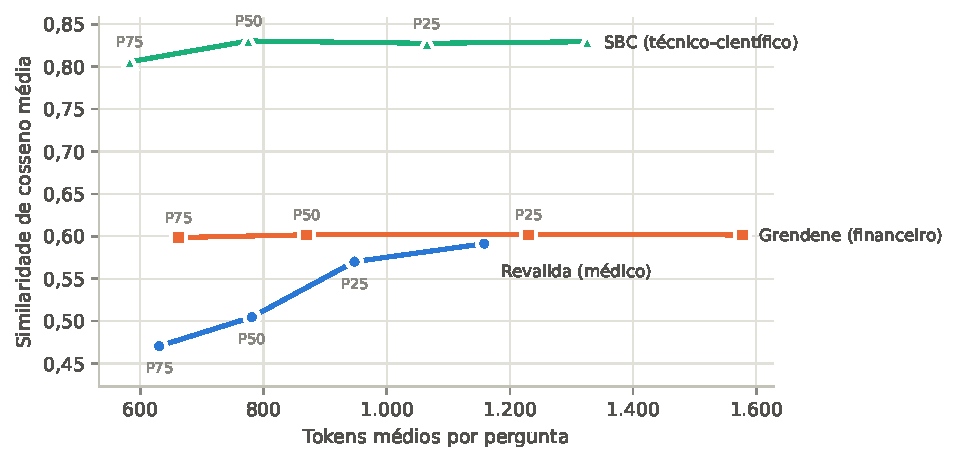
\includegraphics[width=0.75\linewidth]{compressao_calibrada.pdf}
\caption{Compressão contextual com limiares calibrados por domínio: tokens médios e similaridade de cosseno média com limiares nos quantis 25, 50 e 75 da similaridade dos fragmentos recuperados. O ponto mais à direita de cada linha corresponde à execução sem filtro.}
\label{fig:compressao_calibrada}
\end{figure}

\subsection{Bancos vetoriais}
\label{ssc:vectorstores}

A Tabela~\ref{tab:vectorstores} compara ChromaDB e FAISS sobre os mesmos vetores. Os fragmentos recuperados foram idênticos em 100\% das consultas nos três domínios, o que confirma que a escolha do banco, com busca exata, não afeta a qualidade das respostas. Em infraestrutura, o FAISS foi muito mais rápido: entre 0,1 e 0,8 ms para indexar, contra 95 a 425 ms do ChromaDB (500 a 1.700 vezes menos), e entre 0,016 e 0,049 ms por consulta, contra 2,8 a 5,9 ms (60 a 270 vezes menos). O FAISS também alocou menos memória (2,1 MB contra 38,7 MB no maior corpus). Parte dessa diferença, porém, corresponde a funcionalidades que o \texttt{IndexFlatL2} não oferece e o ChromaDB sim: persistência em disco, armazenamento dos textos e filtros por metadados. Em valores absolutos, os tempos do ChromaDB (milissegundos) são desprezíveis diante do tempo de geração (segundos).

\tabela{vectorstores}

\section{Discussão}
\label{sc:discussao}

\subsection{Qual método escolher}

Em relação à QP1, nenhum método se destaca estatisticamente pela similaridade de cosseno: as diferenças entre os seis são pequenas diante da variação entre perguntas, e a ordenação muda de domínio para domínio. Pela \emph{Answer Relevancy} há diferenças significativas, e em custo as diferenças são grandes e estáveis. Nessas condições, as recomendações mais sólidas são de exclusão. O Reciprocal custa cerca de cinco vezes o Stuff em tokens, tem a pior \emph{Answer Relevancy} e fica no grupo intermediário em similaridade: no conjunto das perguntas, não compensa o custo adicional. O Query Step-Down teve a maior \emph{Answer Relevancy}, mas sem diferença significativa em relação ao Map-Reduce, que usa cerca de um terço dos tokens (1.987 contra 6.773 por pergunta).

Entre os métodos restantes, a escolha depende do que se entende por qualidade. O Map-Reduce foi o mais equilibrado: segundo em \emph{Answer Relevancy}, intermediário em similaridade e com custo de 1,5 vez o Stuff. O Map-Rerank, com o mesmo custo, produz respostas curtas e diretas, o que lhe deu a maior similaridade média e uma das piores \emph{Answer Relevancy}. Ele é adequado quando a resposta esperada é um valor único, como nas perguntas financeiras, e menos quando se espera uma resposta explicativa. O Refine teve a maior \emph{Faithfulness} bruta, sem diferença significativa, a um custo de 1,9 vez o Stuff. O Stuff continua sendo a opção mais barata e mais rápida, com a ressalva das recusas, discutida a seguir.

Esses resultados divergem em parte do estudo de referência \cite{sakar2025rag}, no qual o Reciprocal RAG obteve a maior similaridade. Aqui ele foi o melhor apenas no domínio financeiro. Três diferenças de desenho podem explicar a divergência: o idioma, o tipo de pergunta (questões discursivas e perguntas factuais sobre documentos longos) e a escala, já que 27 perguntas não permitem detectar diferenças pequenas entre métodos.

\subsection{Recusas explicam boa parte da diferença do Stuff}

A análise das recusas sugere um mecanismo concreto por trás da desvantagem do Stuff. Ele recebe os quatro fragmentos de uma vez, com a instrução de dizer que não sabe quando a resposta não estiver no contexto, e recusou 30\% das perguntas. Excluídas as recusas, sua similaridade fica no mesmo patamar da do Map-Rerank, e sua \emph{Faithfulness} passa a ser a maior entre os métodos. O Map-Rerank, ao avaliar cada fragmento separadamente e reter a resposta de maior confiança, é pouco afetado por recusas: basta um fragmento que sustente uma resposta. As recusas se concentraram no domínio médico, cujas perguntas combinam uma vinheta clínica longa com um enunciado específico e cujo corpus reúne cinco documentos.

Barnett et al.~\cite{barnett2024seven} distinguem dois pontos de falha relevantes aqui: o contexto correto não é recuperado, ou é recuperado e o modelo não consegue extrair dele a resposta. As métricas RAGAS indicam que o segundo caso predominou. Em 10 das 13 recusas, o juiz considerou que o contexto recuperado cobria ao menos metade da resposta de referência, com a ressalva de que o próprio \emph{Context Recall} é uma estimativa ruidosa (Seção~\ref{ssc:disc_juiz}). As recusas também são instáveis: o Stuff foi executado três vezes sobre as mesmas perguntas, com temperatura 0, e em uma delas recusou em uma execução e respondeu corretamente nas outras duas (similaridade de 0,433 contra 0,87). Parte da diferença entre métodos, portanto, pode depender do texto do prompt e de decisões do modelo que estão no limite, e não só da arquitetura. Uma instrução de recusa mais branda aproximaria o Stuff dos demais métodos, possivelmente ao custo de mais respostas sem sustentação no contexto. Isso não foi testado aqui e fica como trabalho futuro.

\subsection{A métrica muda a conclusão}

A resposta à QP2 é afirmativa: a ordenação dos métodos depende da métrica. O Map-Rerank passa do primeiro lugar em similaridade de cosseno para o quinto em \emph{Answer Relevancy}, e o Reciprocal, intermediário no cosseno, fica em último. As correlações linha a linha entre cosseno e as métricas RAGAS são fracas ($\rho$ entre 0,16 e 0,35). O mecanismo é a forma da resposta. O cosseno premia respostas curtas quando a referência também é curta, e penaliza respostas corretas redigidas em frase completa. A \emph{Answer Relevancy} faz o oposto. Nenhuma das duas verifica o valor em si: na pergunta sobre o patrimônio líquido, um número diferente do gabarito obteve similaridade de 0,613.

Isso tem uma consequência para estudos comparativos como o de referência, que usam apenas a similaridade de cosseno: parte da vantagem atribuída a um método pode refletir a forma das respostas que ele produz, e não sua correção. A recomendação que decorre deste trabalho é reportar mais de uma métrica e declarar qual noção de qualidade importa para a aplicação: exatidão de um valor, completude da explicação ou ancoragem no documento. Para respostas numéricas, uma comparação direta do valor extraído seria mais adequada que qualquer métrica baseada em embeddings.

\subsection{Confiabilidade do juiz automático}
\label{ssc:disc_juiz}

A validação do juiz não indicou viés de autopreferência. Nas métricas que avaliam a própria resposta, o \texttt{gpt-4o-mini} foi igualmente ou mais rigoroso com as respostas que gerou do que um juiz de outra família. Isso apoia o uso do mesmo modelo como gerador e juiz neste estudo, como também fizeram Medeiros e Oliveira~\cite{medeiros2025embeddings}, ao menos para as métricas e o modelo avaliados aqui.

A confiabilidade, porém, depende da métrica, e isso determina o que pode ser concluído de cada uma. A \emph{Answer Relevancy} foi estável no reteste e entre juízes, com a mesma ordenação dos métodos. As conclusões baseadas nela, inclusive a inversão em relação ao cosseno discutida acima, são robustas à escolha do juiz. O \emph{Context Recall} também foi estável, o que sustenta a leitura das recusas. A \emph{Faithfulness} variou de forma considerável mesmo quando o mesmo juiz avaliou duas vezes a mesma resposta, e os juízes divergiram no tratamento das recusas. As diferenças de \emph{Faithfulness} entre métodos, que já não eram significativas, não devem ser interpretadas além disso. A \emph{Context Precision} não foi confiável: os juízes não concordaram entre si, e a mesma entrada recebeu notas diferentes em avaliações repetidas. Como ela avalia a recuperação, que é idêntica entre os métodos, isso não afeta a comparação entre eles, mas seus valores absolutos não devem ser tomados como medida da qualidade da recuperação.

Do ponto de vista metodológico, a validação custou pouco: 54 respostas reavaliadas por dois juízes. Estudos que usam LLMs como juízes com um único modelo e uma única execução por resposta tratam como medida o que, em parte, é ruído do juiz. Um reteste numa amostra e a comparação com um juiz independente indicam quais métricas sustentam conclusões e quais não.

\subsection{Compressão contextual}

Em relação à QP3, os limiares fixos não se mostraram transferíveis. Com o BGE-M3, a similaridade dos fragmentos recuperados ficou concentrada numa faixa estreita, entre 0,52 e 0,75. Limiares abaixo dela, como 0,3 e 0,5, não têm efeito; limiares acima, como 0,7, reduzem o contexto a um único fragmento. Valores definidos para outros modelos de embedding, como os do estudo de referência, não se aplicam diretamente, porque a escala de similaridade é própria de cada modelo. A calibração pelos quantis da distribuição observada resolve esse problema: transforma o limiar em uma fração aproximada de fragmentos descartados e produz um compromisso gradual entre tokens e qualidade.

Os valores calibrados foram parecidos nos três domínios (quantil 50 entre 0,626 e 0,639), o que sugere que, para um mesmo embedding, a distribuição de similaridade é relativamente estável. O que variou foi o quanto cada domínio depende dos fragmentos descartados. Nos domínios financeiro e técnico-científico, com um único documento cada, descartar metade dos fragmentos economizou mais de 40\% dos tokens sem perda de similaridade. No domínio médico, em que a resposta pode depender de fragmentos de documentos diferentes e as perguntas são longas, cada fragmento descartado custou qualidade. A recomendação prática é calibrar o limiar em uma amostra de perguntas do domínio de interesse e validar a qualidade antes de adotá-lo. Como aqui a calibração usou as mesmas perguntas avaliadas, os ganhos observados são um limite superior do que se obteria com um limiar escolhido de antemão.

\subsection{Bancos vetoriais}

Em relação à QP4, a comparação confirma que, com busca exata e a mesma métrica de distância, o banco vetorial não altera a qualidade das respostas: os fragmentos recuperados foram idênticos. O FAISS foi muito mais rápido e econômico em memória, mas os tempos do ChromaDB, de poucos milissegundos, são desprezíveis diante dos segundos gastos na geração. Para corpora do tamanho dos usados aqui, de dezenas a centenas de fragmentos, a persistência e os filtros por metadados do ChromaDB custam pouco. A vantagem do FAISS tende a importar em corpora ordens de grandeza maiores ou com alto volume de consultas, cenários que não foram avaliados.

\subsection{Limitações}

Os resultados devem ser lidos à luz das seguintes limitações.

\begin{itemize}
  \item \textbf{Tamanho da amostra.} São 27 perguntas no total e de 7 a 12 por domínio. Isso basta para medir diferenças de custo, que são grandes, mas não para detectar diferenças moderadas de qualidade entre métodos.
  \item \textbf{Configuração fixa.} Um único LLM (\texttt{gpt-4o-mini}), um único embedding (BGE-M3), um único tamanho de fragmento e $k = 4$. As conclusões valem para essa configuração. Com um LLM mais capaz, por exemplo, a taxa de recusas e a vantagem do Map-Rerank poderiam ser diferentes.
  \item \textbf{Perguntas redigidas pelos autores.} Nos domínios financeiro e técnico-científico, as perguntas e as respostas de referência foram redigidas pelos autores, ainda que ancoradas em trechos literais. Só o domínio médico tem gabarito oficial externo.
  \item \textbf{Extração de texto.} Os PDFs foram convertidos em texto simples, e tabelas financeiras perdem parte da estrutura nessa conversão, o que afeta a recuperação de valores numéricos.
  \item \textbf{Métricas automáticas.} A similaridade de cosseno depende da forma da resposta, e as métricas RAGAS dependem de um juiz LLM não determinístico (Seção~\ref{ssc:disc_juiz}). Nenhuma das duas foi validada contra avaliação humana.
  \item \textbf{Determinismo da geração.} Mesmo com temperatura 0, a geração não é totalmente determinística. O Stuff sem filtro foi executado três vezes sobre as 27 perguntas (no comparativo e nas duas rodadas de compressão), e 21 respostas saíram idênticas nas três execuções. Cada resultado reportado vem de uma única execução por pergunta e método.
  \item \textbf{Custo de hardware.} Como a geração ocorre em uma API remota, as medidas locais de CPU e memória não refletem o custo de inferência dos métodos. O custo foi medido em tokens e tempo, e a comparação de hardware se restringiu aos bancos vetoriais.
  \item \textbf{Versão do modelo.} Os registros armazenaram o apelido do modelo, e não a versão exata, o que dificulta a reprodução exata caso o apelido passe a apontar para outra versão.
\end{itemize}

\section{Conclusão}
\label{sc:conclusao}

Este trabalho replicou, com documentos em português, o desenho comparativo de Şakar e Emekci~\cite{sakar2025rag} para seis métodos de RAG, em três domínios brasileiros com respostas de referência verificáveis: o Revalida 2024/2 (médico), as Informações Trimestrais da Grendene S.A. (financeiro) e um artigo científico sobre RAG em português (técnico-científico). Além da similaridade de cosseno usada pelo estudo de referência, as respostas foram avaliadas com as métricas RAGAS, e o juiz automático foi validado contra ele mesmo e contra um juiz de outra família de modelos.

Os principais resultados são os seguintes:

\begin{enumerate}
  \item \textbf{Custo separa os métodos; qualidade, não.} Em similaridade de cosseno, nenhum método foi estatisticamente superior, e o melhor método variou entre os domínios. Em custo, as diferenças foram grandes: Query Step-Down e Reciprocal usaram cerca de cinco vezes os tokens do Stuff sem qualidade superior. O Reciprocal, melhor método no estudo de referência, não compensou o custo adicional no conjunto das perguntas: foi o melhor apenas no domínio financeiro e teve a pior \emph{Answer Relevancy}.
  \item \textbf{A métrica muda a ordenação.} O Map-Rerank, com a maior similaridade de cosseno, ficou entre os piores em \emph{Answer Relevancy}, e as correlações entre as métricas foram fracas. As duas métricas reagem à forma da resposta, curta ou explicativa, e nenhuma verifica diretamente se um valor está correto.
  \item \textbf{Recusas pesam.} O Stuff recusou 30\% das perguntas, na maior parte das vezes com a informação presente no contexto, segundo o juiz. Sem as recusas, sua similaridade fica próxima da do Map-Rerank e sua \emph{Faithfulness} média é a maior entre os métodos.
  \item \textbf{Compressão precisa de calibração.} Limiares fixos de similaridade ou não descartaram nada, ou descartaram quase tudo. Limiares calibrados pela distribuição observada cortaram cerca de 40\% dos tokens sem perda de similaridade em dois dos três domínios.
  \item \textbf{O banco vetorial é questão de infraestrutura.} ChromaDB e FAISS recuperaram exatamente os mesmos fragmentos. O FAISS foi muito mais rápido, mas os tempos de ambos são desprezíveis diante da geração nos corpora avaliados.
\end{enumerate}

Quanto à avaliação automática, a validação não indicou viés de autopreferência do \texttt{gpt-4o-mini} como juiz, mas mostrou que a confiabilidade das métricas RAGAS varia muito: \emph{Answer Relevancy} e \emph{Context Recall} foram estáveis entre execuções e entre juízes, a \emph{Faithfulness} foi moderadamente estável, e a \emph{Context Precision} não foi confiável.

Do ponto de vista prático, o trabalho sugere quatro diretrizes para quem constrói sistemas RAG sobre documentos em português: escolher o método pelo custo e pelo tipo de resposta esperada, e não por uma ordenação geral de qualidade; avaliar com mais de uma métrica e declarar qual noção de qualidade importa para a aplicação; ao usar um LLM como juiz, verificar a estabilidade de cada métrica com um reteste e um juiz independente antes de tirar conclusões dela; e calibrar filtros de compressão na distribuição de similaridade do próprio embedding e domínio.

Como trabalhos futuros, destacam-se: ampliar o número de perguntas por domínio para dar poder estatístico às comparações de qualidade; variar o LLM e o modelo de embedding, retomando o eixo previsto no plano original; testar instruções de recusa mais brandas no prompt; validar as métricas automáticas contra avaliação humana; e avaliar o desempenho dos bancos vetoriais em corpora maiores.


\renewcommand\refname{Referências}
\bibliographystyle{IEEEtran}
\bibliography{referencias}

\end{document}
